\section{Pruebas de rango de medición mínimo}
\begin{figure}[H]
	\centering
	\begin{subfigure}{0.6\textwidth}
		\centering
		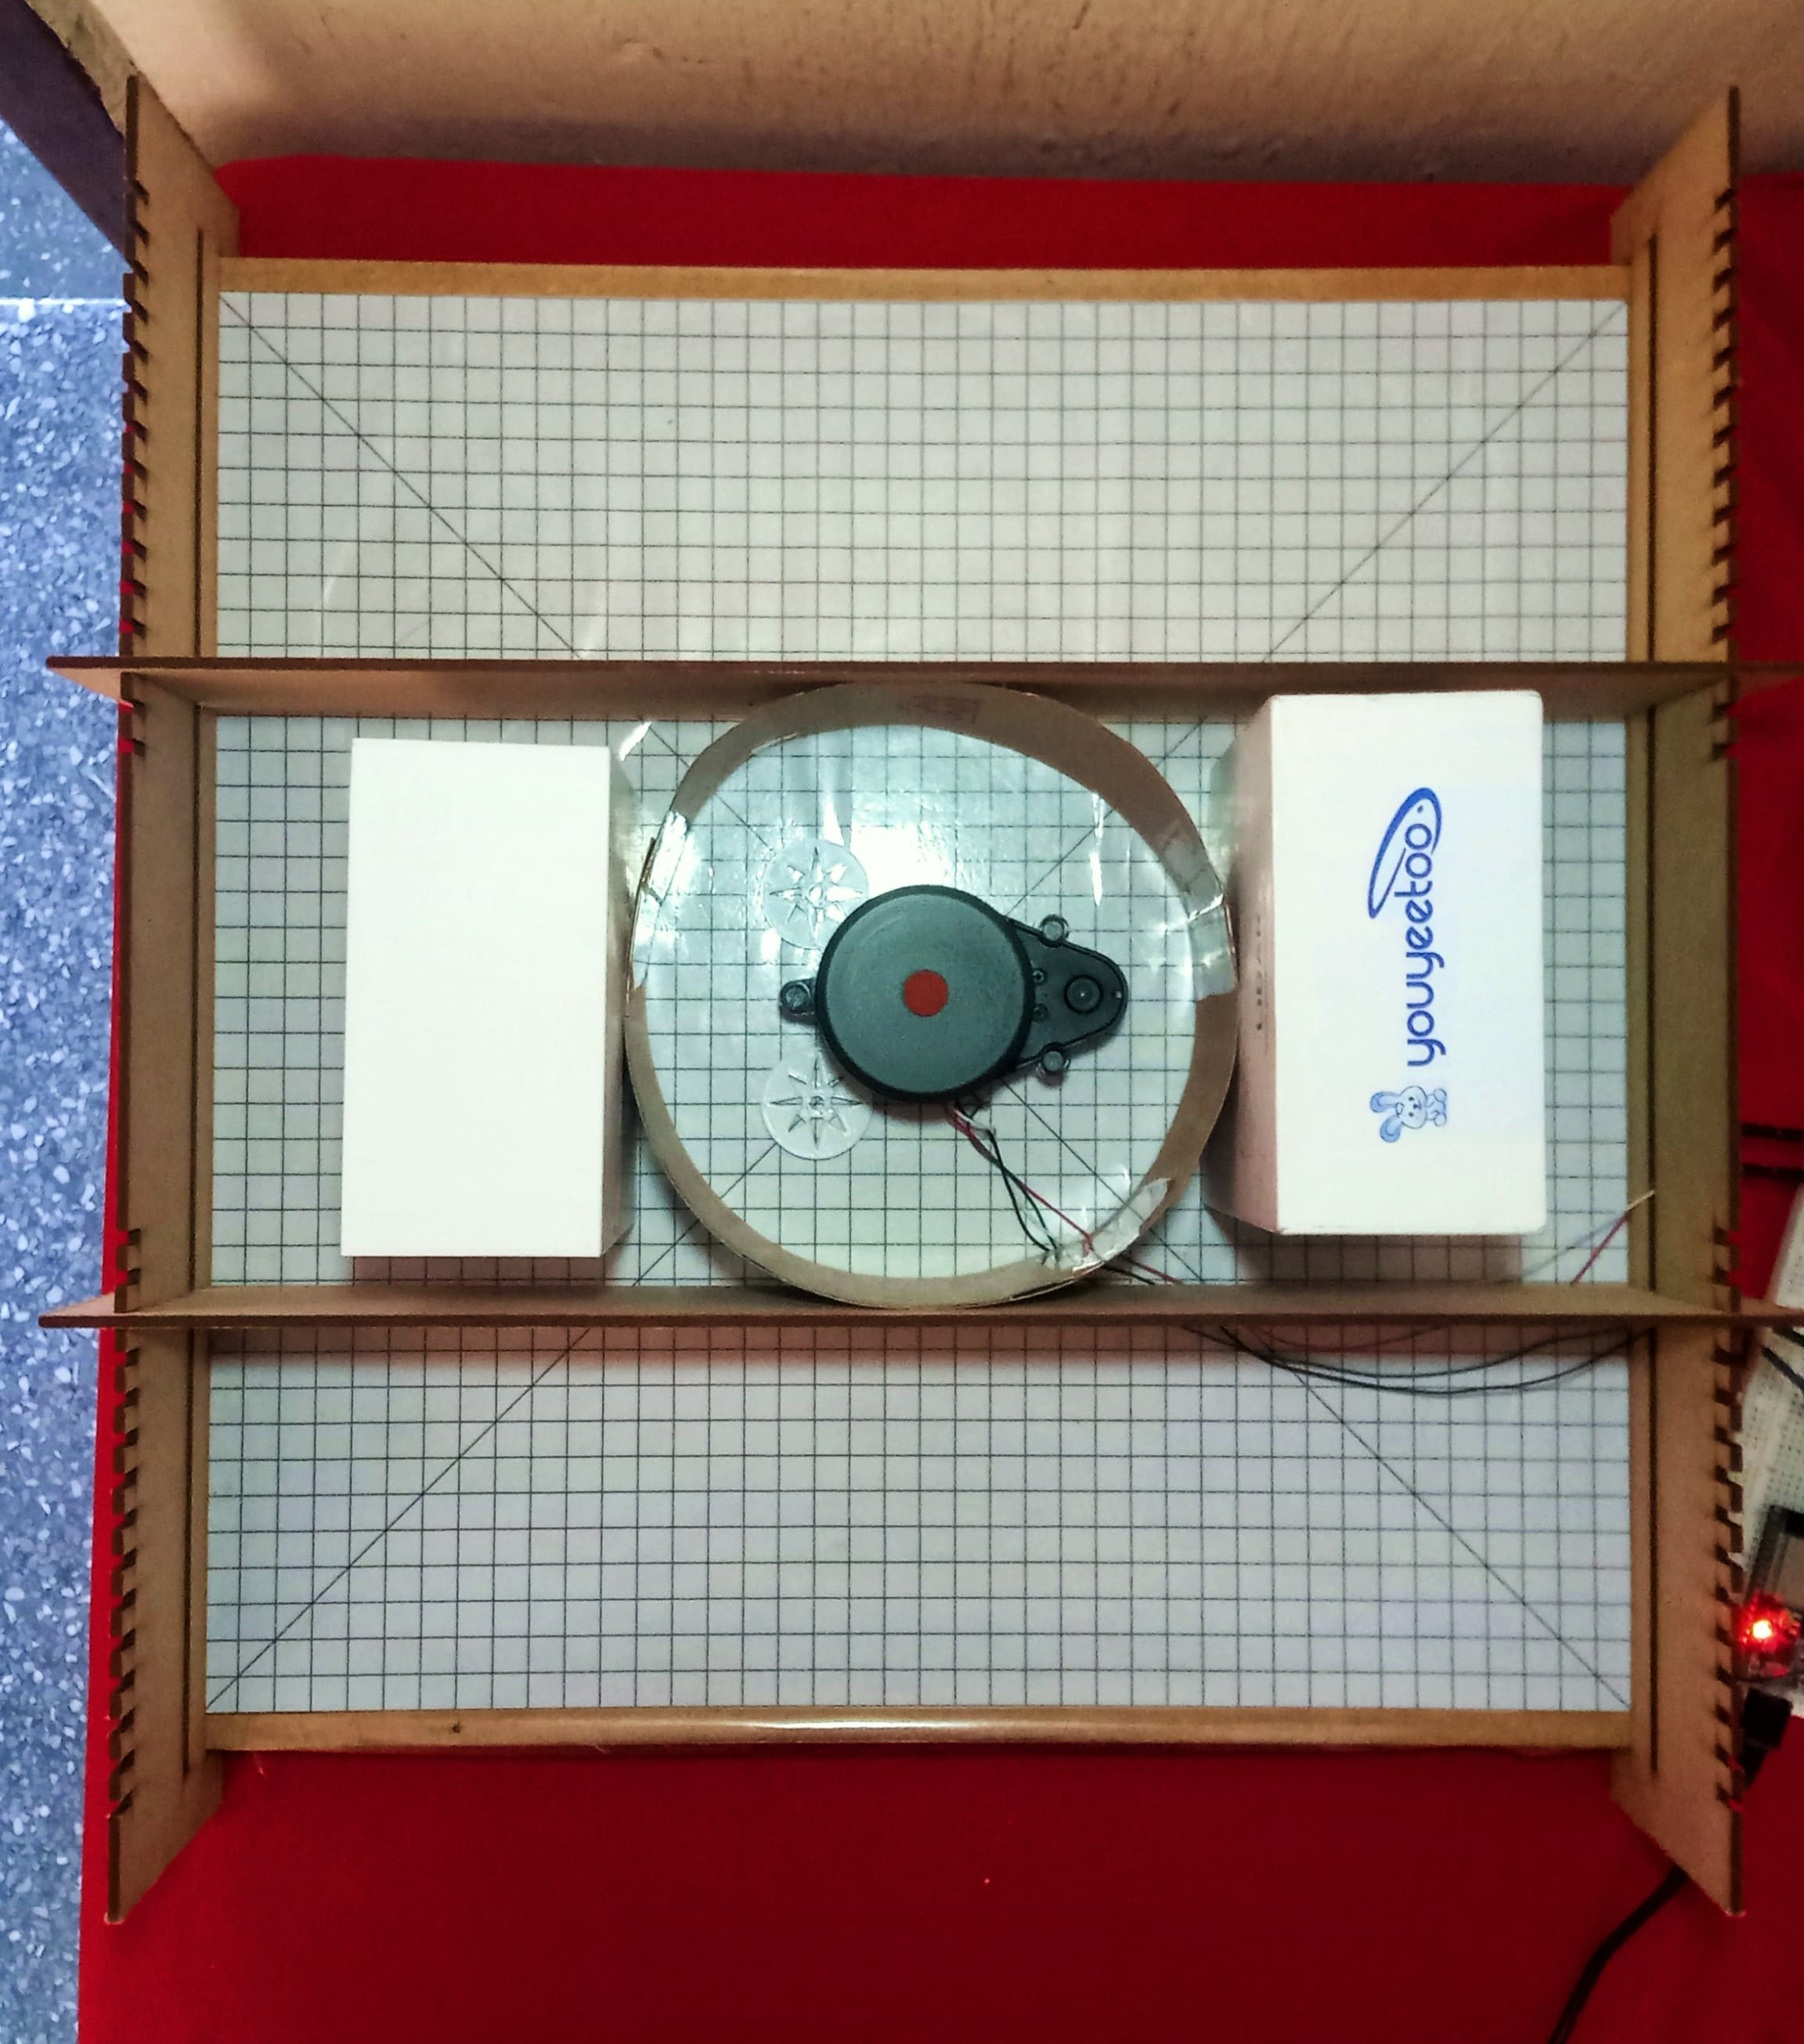
\includegraphics[width=0.5\linewidth]{disposicion_lidar5.jpeg}
		\caption{Disposición del sensor FHL-LD20 dentro del entorno circular: 7 cm de radio}
		\label{disposicion_lidar5}
		\vspace{1em}
	\end{subfigure}
	\begin{subfigure}{0.45\textwidth}
		\centering
		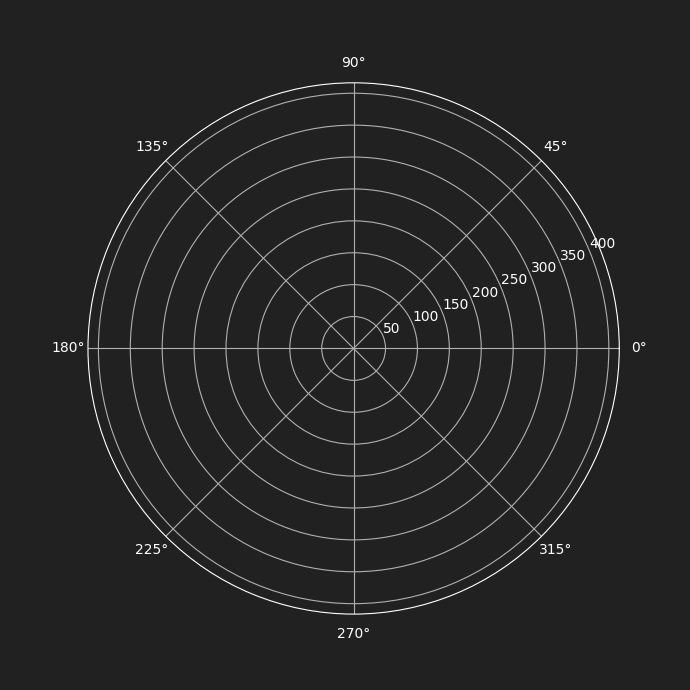
\includegraphics[width=0.7\linewidth]{try_7cm_r.png}
		\caption{Reconstrucción en coordenadas polares de tres revoluciones completas de lectura en entorno circular: 7 cm de radio}
		\label{try_7cm_r}
	\end{subfigure}
	\hspace{1em}
	\begin{subfigure}{0.45\textwidth}
		\centering
		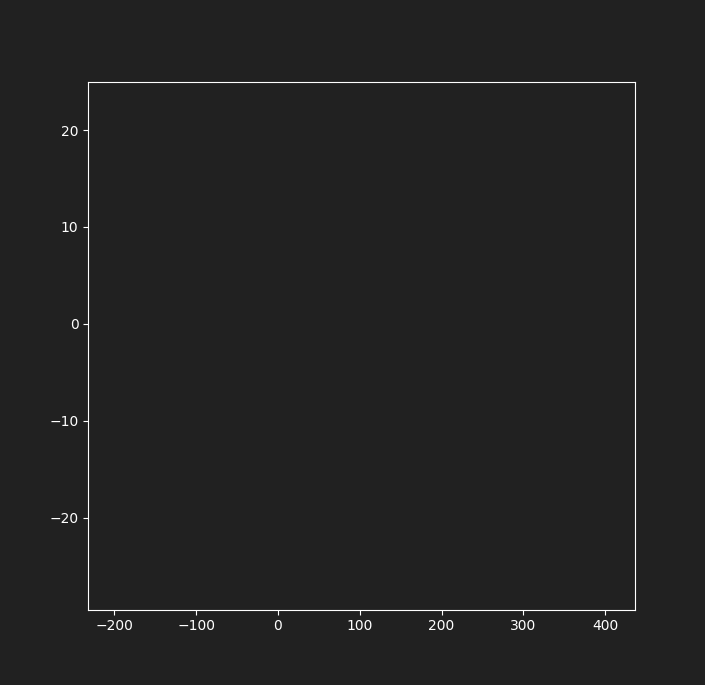
\includegraphics[width=0.7\linewidth]{try_7cm_r_car.png}
		\caption{Reconstrucción en coordenadas cartesianas de tres revoluciones completas de lectura en entorno circular: 7 cm de radio}
		\label{try_7cm_r_car}
	\end{subfigure}
	\caption{Reconstrucciones vacías de tres revoluciones completas de lectura en entorno circular: 7 cm de radio}
	\label{fig: reconstrucciones_vacías_7}
\end{figure}

\begin{figure}[H]
	\centering
	\begin{subfigure}{0.6\textwidth}
		\centering
		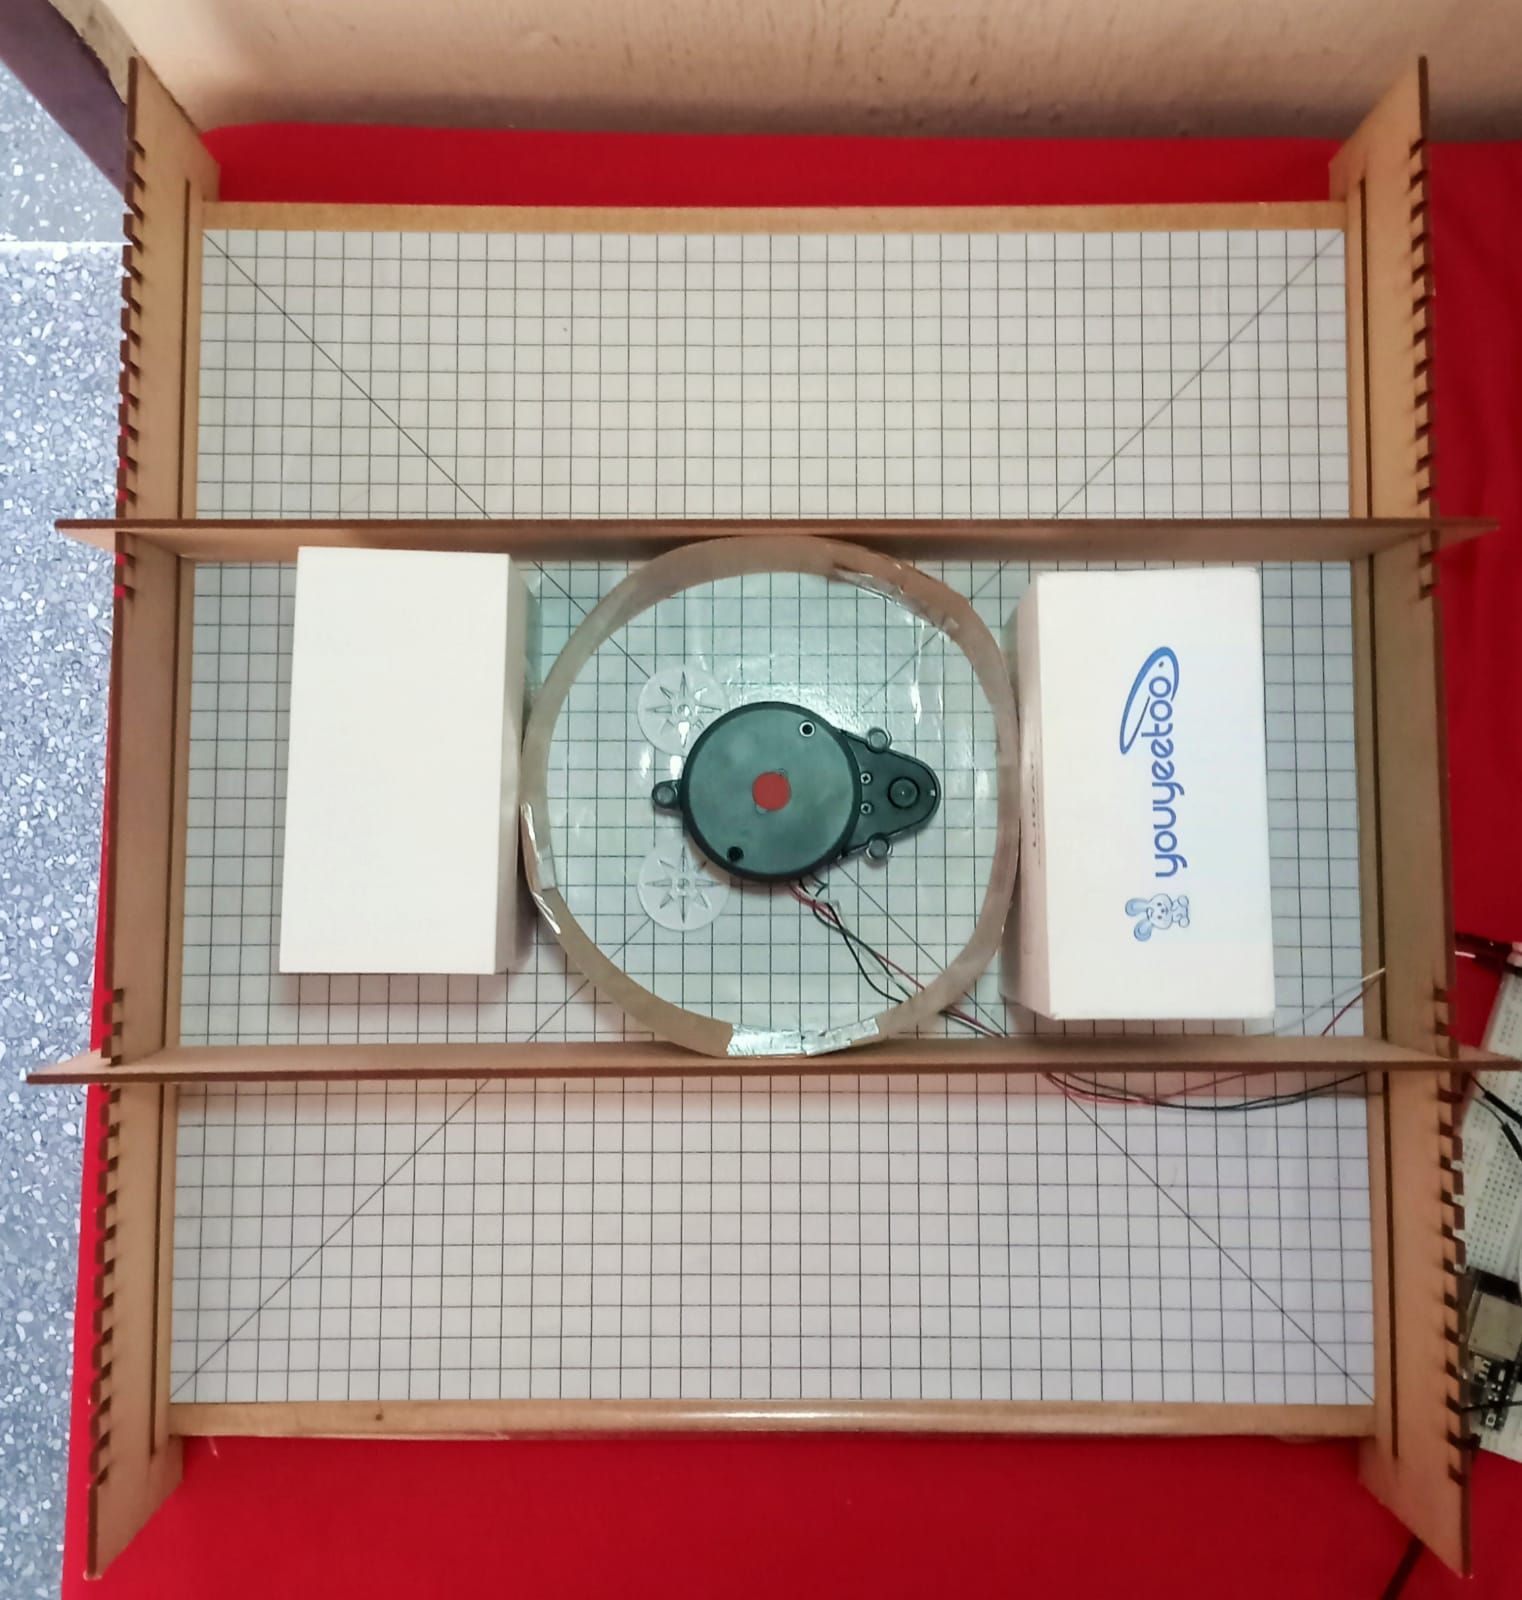
\includegraphics[width=0.6\linewidth]{disposicion_lidar6.jpeg}
		\caption{Disposición del sensor FHL-LD20 dentro del entorno circular: 8 cm de radio}
		\label{disposicion_lidar6}
		\vspace{1em}
	\end{subfigure}
	\begin{subfigure}{0.45\textwidth}
		\centering
		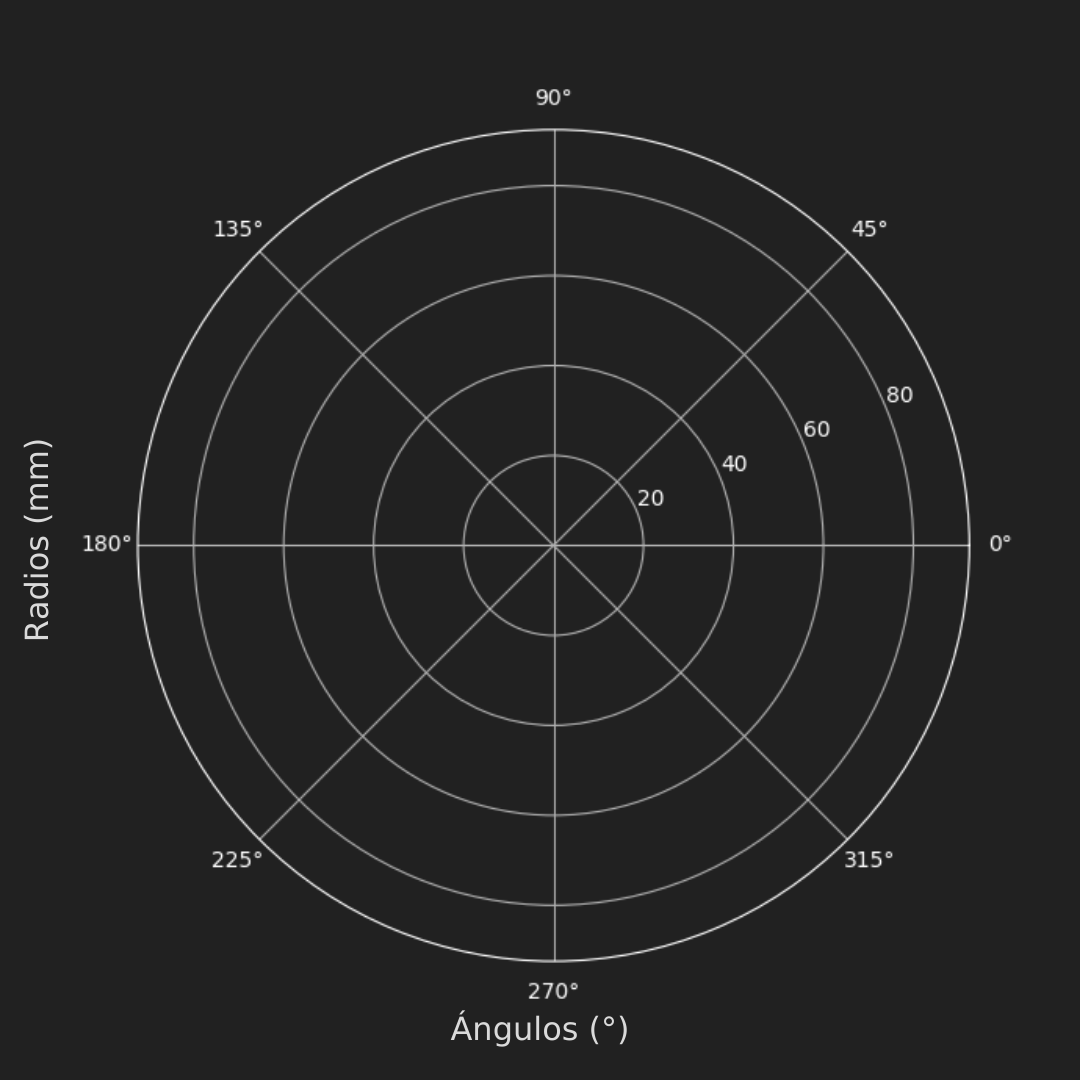
\includegraphics[width=0.8\linewidth]{try_8cm_r.png}
		\caption{Reconstrucción en coordenadas polares de tres revoluciones completas de lectura en entorno circular: 8 cm de radio}
		\label{try_8cm_r}
	\end{subfigure}
	\hspace{1em}
	\begin{subfigure}{0.45\textwidth}
		\centering
		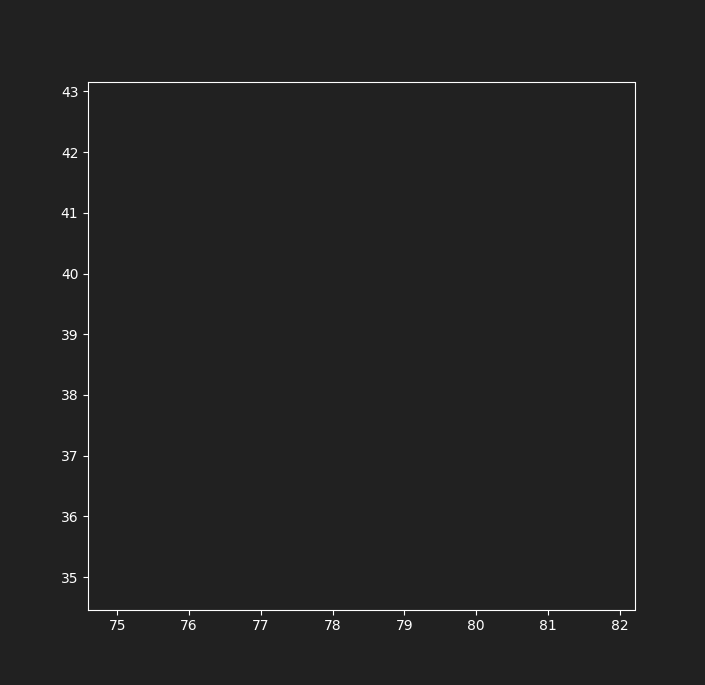
\includegraphics[width=0.8\linewidth]{try_8cm_r_car.png}
		\caption{Reconstrucción en coordenadas cartesianas de tres revoluciones completas de lectura en entorno circular: 8 cm de radio}
		\label{try_8cm_r_car}
	\end{subfigure}
	\caption{Reconstrucciones vacías de tres revoluciones completas de lectura en entorno circular: 8 cm de radio}
	\label{fig: reconstrucciones_vacías_8}
\end{figure}


\begin{figure}[H]
	\centering
	\begin{subfigure}{0.6\textwidth}
		\centering
		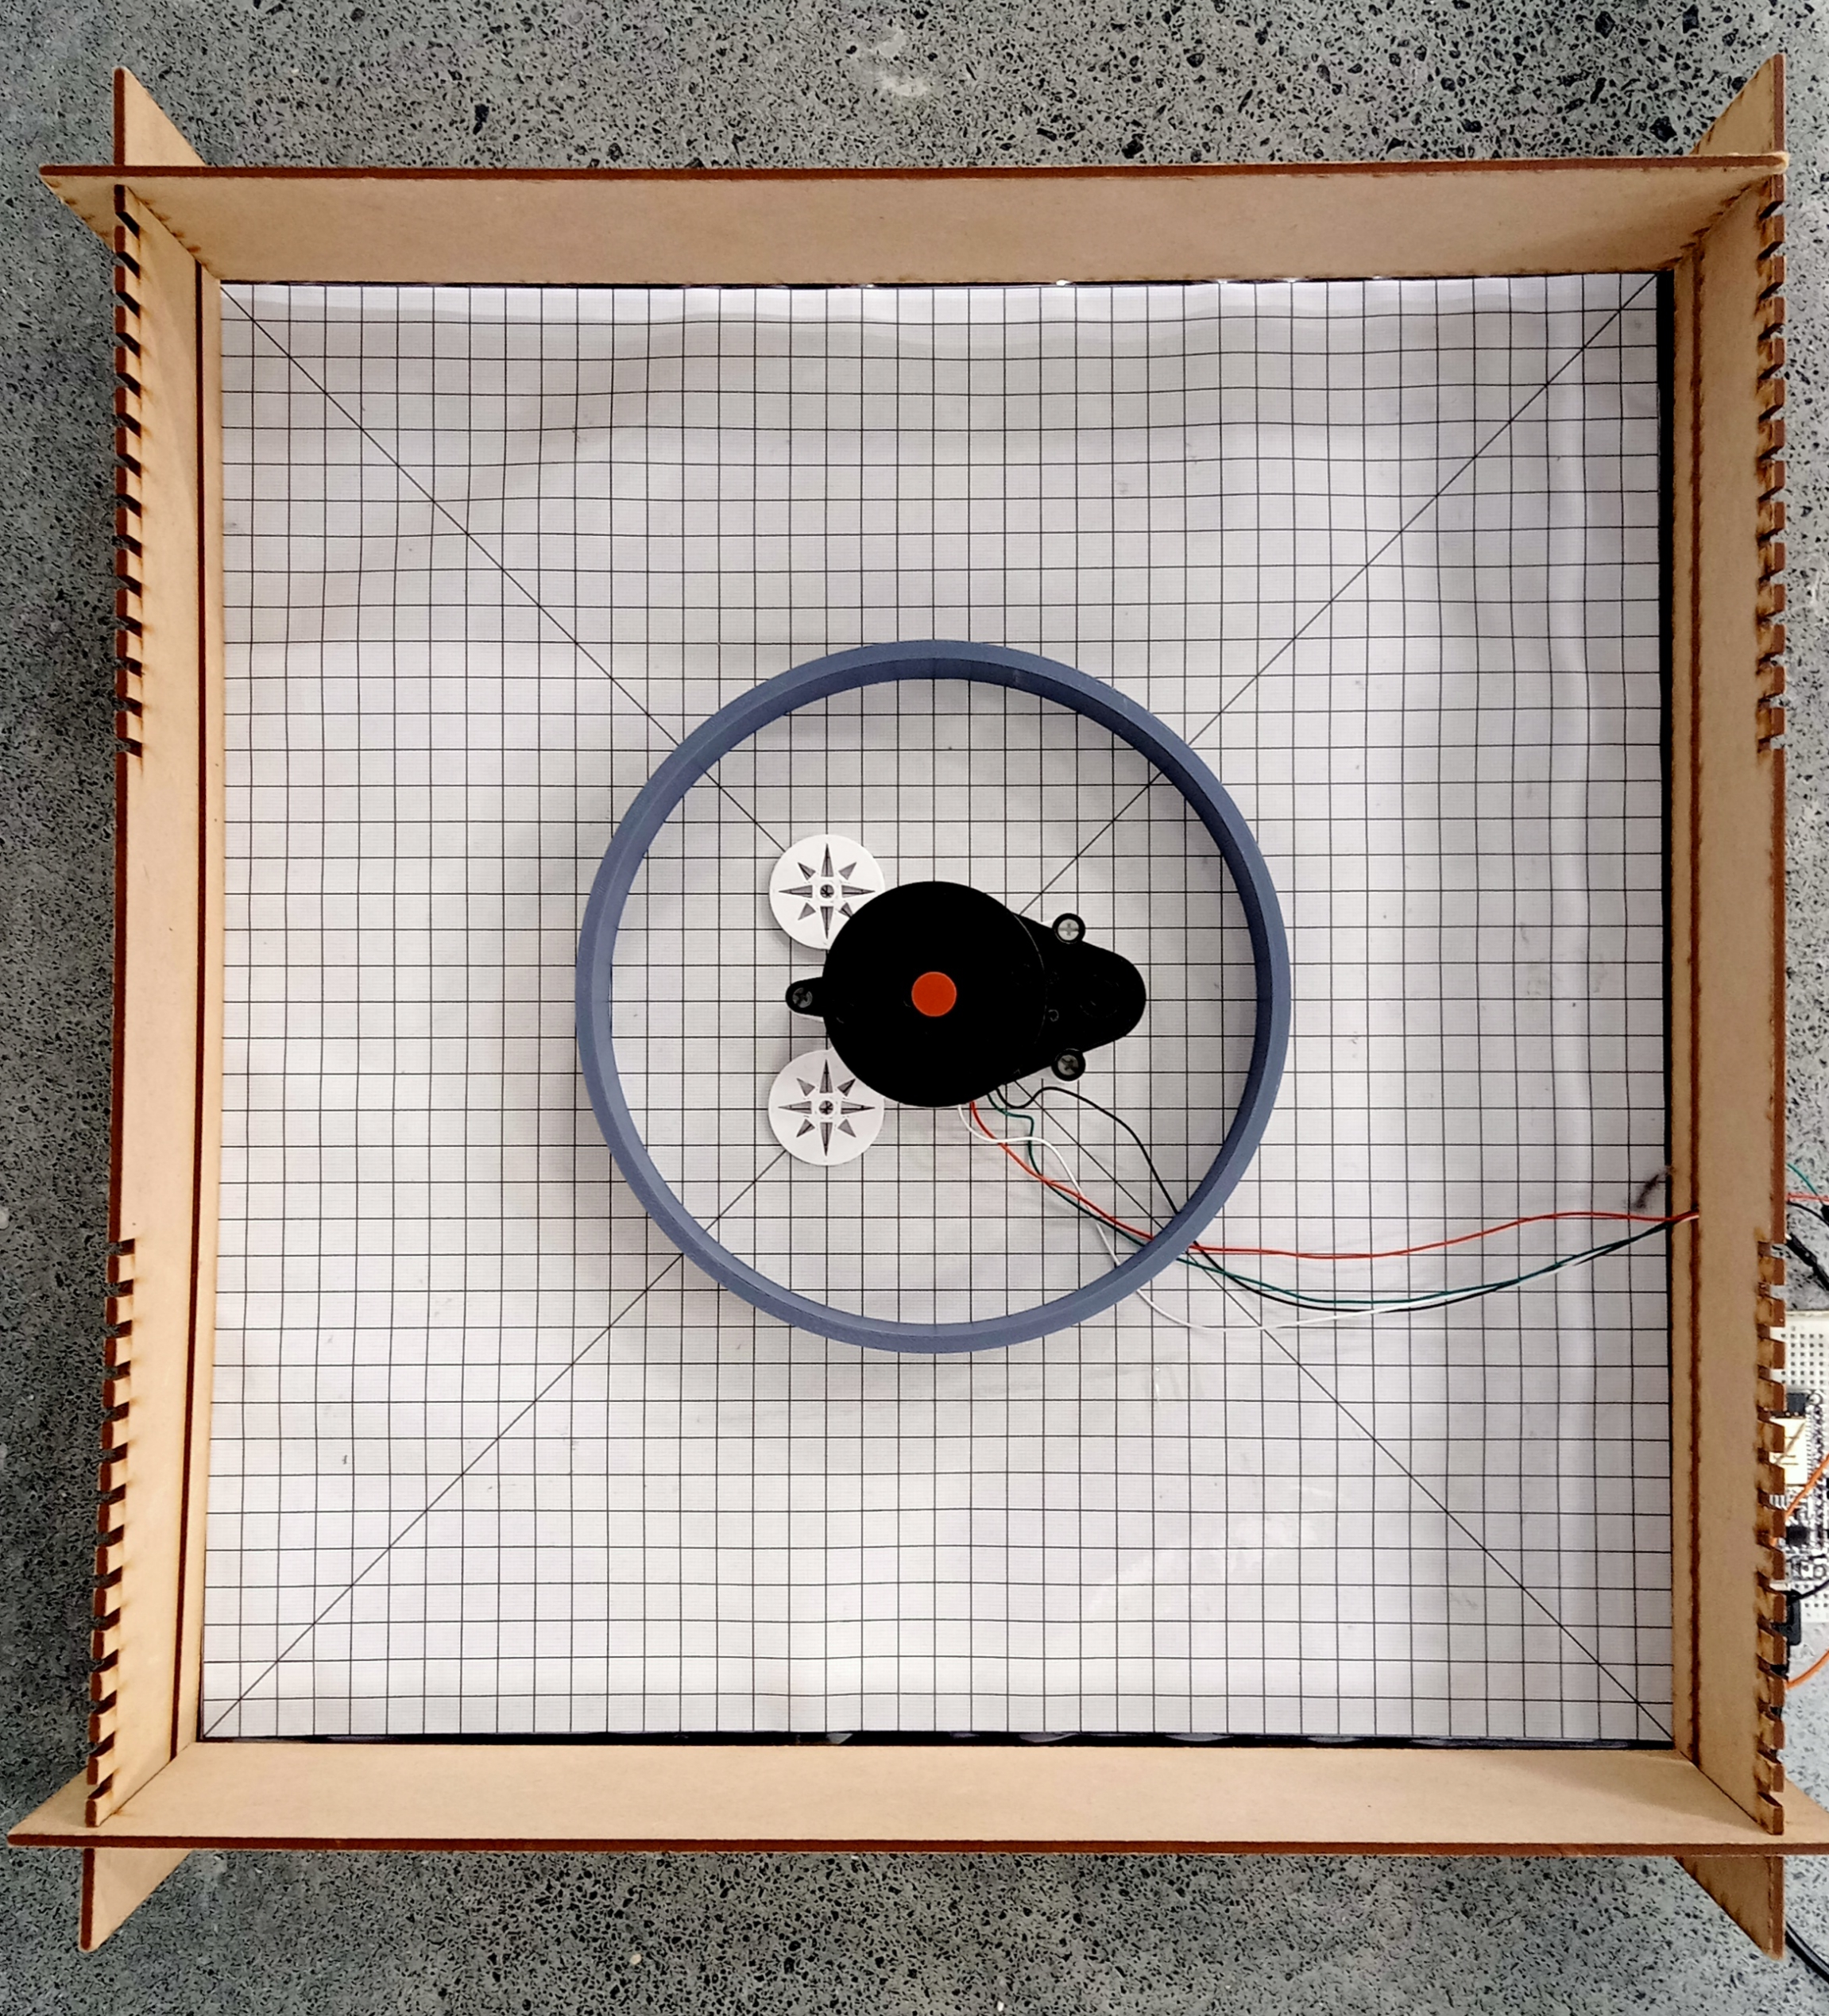
\includegraphics[width=0.6\linewidth]{disposicion_lidar7.jpeg}
		\caption{Disposición del sensor FHL-LD20 dentro del entorno circular: 9 cm de radio}
		\label{disposicion_lidar6}
		\vspace{1em}
	\end{subfigure}
	\begin{subfigure}{0.45\textwidth}
		\centering
		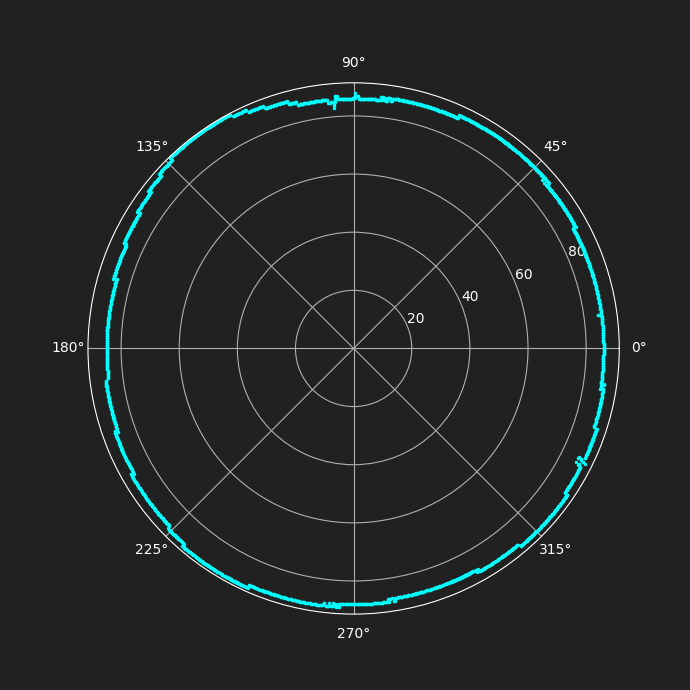
\includegraphics[width=0.8\linewidth]{try_9cm_r.png}
		\caption{Reconstrucción en coordenadas polares de tres revoluciones completas de lectura en entorno circular: 9 cm de radio}
		\label{try_9cm_r}
	\end{subfigure}
	\hspace{1em}
	\begin{subfigure}{0.45\textwidth}
		\centering
		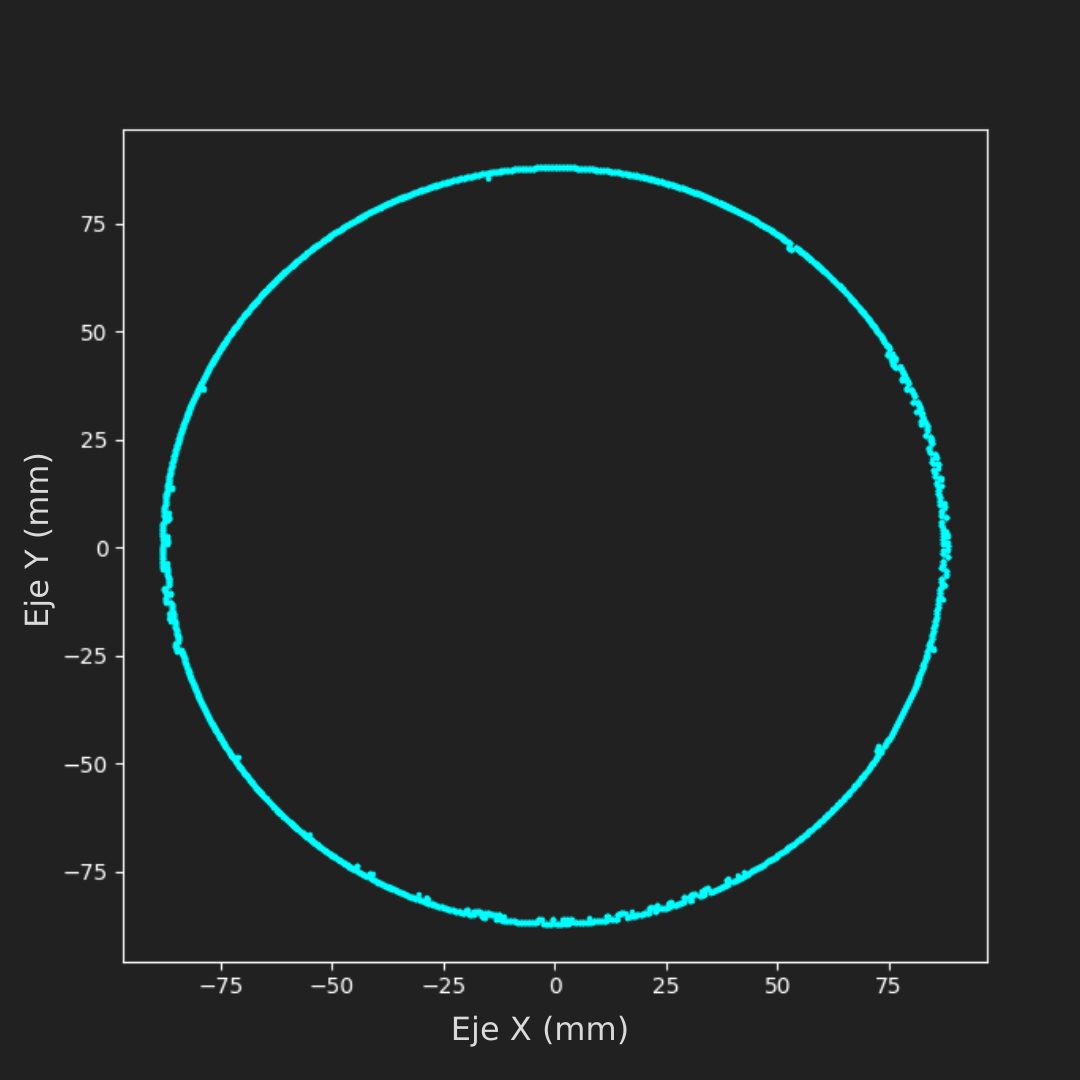
\includegraphics[width=0.8\linewidth]{try_9cm_r_car.png}
		\caption{Reconstrucción en coordenadas cartesianas de tres revoluciones completas de lectura en entorno circular: 9 cm de radio}
		\label{try_9cm_r_car}
	\end{subfigure}
	\caption{Reconstrucciones vacías de tres revoluciones completas de lectura en entorno circular: 9 cm de radio}
	\label{fig: reconstrucciones_vacías_9}
\end{figure}

\section{Pruebas para la estimación de la varianza asociada a las mediciones de distancia del sensor}
